\documentclass[letterpaper,11pt]{article}

\usepackage{amsmath, amsfonts, amscd, amssymb, amsthm}
\usepackage{graphicx}
%\usepackage{import}
\usepackage{versions}
\usepackage{crop}
\usepackage{multicol}
\usepackage{makeidx}
\usepackage{hyperref}
\usepackage{ifthen}
\usepackage[format=hang,font=normalsize,labelfont=bf]{caption}
\usepackage{natbib}
\usepackage{setspace}
\usepackage{placeins}
\usepackage{framed}
\usepackage{enumitem}
\usepackage{geometry}
\geometry{letterpaper,tmargin=1in,bmargin=1in,lmargin=1in,rmargin=1in}
\usepackage{multirow}
\usepackage[table]{xcolor}
\usepackage{array}
\usepackage{delarray}
\usepackage{lscape}
\usepackage{float,color, colortbl}
%\usepackage[pdftex]{graphicx}
\usepackage{hyperref}
%\usepackage{tabu}
\usepackage{appendix}
\usepackage{listings}
\usepackage{exercise}
\usepackage{multirow}
\usepackage{tabularx}
\usepackage{booktabs}
\usepackage{threeparttablex}
\usepackage{tablefootnote}

\include{thmstyle}
\bibliographystyle{aer}
\providecommand{\abs}[1]{\lvert#1\rvert}
\providecommand{\norm}[1]{\lVert#1\rVert}
\newcommand{\ve}{\epsilon}
\newcommand{\ip}[2]{\langle #1,#2 \rangle}

\hypersetup{colorlinks,linkcolor=red,urlcolor=blue,citecolor=red}
\theoremstyle{definition}
\newtheorem{theorem}{Theorem}
\newtheorem{acknowledgement}[theorem]{Acknowledgement}
\newtheorem{algorithm}[theorem]{Algorithm}
\newtheorem{axiom}[theorem]{Axiom}
\newtheorem{case}[theorem]{Case}
\newtheorem{claim}[theorem]{Claim}
\newtheorem{conclusion}[theorem]{Conclusion}
\newtheorem{condition}[theorem]{Condition}
\newtheorem{conjecture}[theorem]{Conjecture}
\newtheorem{corollary}[theorem]{Corollary}
\newtheorem{criterion}[theorem]{Criterion}
\newtheorem{definition}{Definition} % Number definitions on their own
\newtheorem{derivation}{Derivation} % Number derivations on their own
\newtheorem{example}[theorem]{Example}
\newtheorem{lemma}[theorem]{Lemma}
\newtheorem{notation}[theorem]{Notation}
\newtheorem{problem}[theorem]{Problem}
\newtheorem{proposition}{Proposition} % Number propositions on their own
\newtheorem{remark}[theorem]{Remark}
\newtheorem{solution}[theorem]{Solution}
\newtheorem{summary}[theorem]{Summary}
%\numberwithin{equation}{document}
\graphicspath{{./Figures/}}
\renewcommand\theenumi{\roman{enumi}}
\DeclareMathOperator*{\argmin}{arg\,min}

\crop
\makeindex


\begin{document}

\begin{titlepage}
	\title{Open Source Macroeconomics Laboratory Boot Camp \\ Week 5 Econ Homework}
	\author{Ruby Zhang}
	\date{\LARGE{2017}}
	\maketitle
\end{titlepage}

\begin{spacing}{1.5}


\section*{DSGE}\label{DSGE_HW}

	% 1
	\begin{Exercise} \label{DSGE_HW_BM_FindA}
		For the Brock and Mirman model, find the value of $A$ in the policy function.  Show that your value is correct.

		For this case find an algebraic solution for the policy function, $k_{t+1} = \Phi (k_t,z_t)$.  Couple of good sources for hints are \citet[exercise 2.2, p. 12]{StokeyLucas1989} and \citet[exercise 1.1, p. 47]{Sargent1987}.
	\end{Exercise}

	Let us guess and verify that the policy function for the Brock and Mirman model is $k_{t+1}=\phi(k_t, z_t) = Ae^{z_t}k_t^{\alpha}$ by using the Euler equation for the Brock and Mirman model:
	\begin{equation*}
		\frac{1}{e^{z_t}k_t^\alpha-k_{t+1}} = \beta E_t\{\frac{\alpha e^{z_{t+1}} k_{t+1}^{\alpha-1}}{e^{z_{t+1}}k_{t+1}^\alpha-k_{t+2}}\}
	\end{equation*}

	Left side of the equation:
	\begin{align*}
		\frac{1}{e^{z_t}k_t^\alpha-Ae^{z_t}k_t^{\alpha}} &= \frac{1}{e^{z_t}k_t^{\alpha}(1-A)}
	\end{align*}
	Right side of the equation (note that the expected $z_{t+1} = \rho z_t$):
	\begin{align*}
		\beta E_t\{\frac{\alpha e^{z_{t+1}} k_{t+1}^{\alpha-1}}{e^{z_{t+1}}k_{t+1}^\alpha-k_{t+2}}\} &= \beta(\frac{\alpha e^{\rho z_t}(Ae^{z_t}k_t^\alpha)^{\alpha-1}}{e^{\rho z_t}(Ae^{z_t}k_t^\alpha)^{\alpha}(1-A)}) \\
		&= \frac{\alpha\beta}{Ae^{z_t}k_t^\alpha(1-A)}
	\end{align*}

	Since the left-hand side and right-hand side must equal each other, $\frac{\alpha\beta}{A} = 1 \Longrightarrow A = \alpha\beta$. Therefore the policy function is $\phi(k_t,z_t) = \alpha\beta e^{z_t}k_t^\alpha$.

	% 2
	\begin{Exercise} \label{DSGE_HW_CharEq_Ln}
		For the model in section \ref{DSGE_BaselineDSGE} of the notes consider the following functional forms:
		\begin{equation}\label{DSGE_HW_CharEq_Ln_eq01}
		\begin{split}
		u(c_t,\ell_t) & = \text{ln }c_t + a \text{ ln }(1-\ell_t)\\
		F(K_t,L_t,z_t) & = e^{z_t}K^{\alpha}_t L^{1-\alpha}_t  \nonumber
		\end{split}
		\end{equation}
		Write out all the characterizing equations for the model using these functional forms.

		Can you use the same tricks as in Exercise 1 to solve for the policy function in this case?  Why or why not?
	\end{Exercise}

	Using the equilibrium given in section 3 we have the following characterizing equations for the given functional forms:
	\begin{align*}
		\ell_t &= L_t \\
		k_t &= K_t \\
		w_t &= W_t \\
		r_t &= R_t \\
		c_t &= (1-\tau)[w_t\ell_t+(r_t-\delta)k_t]+k_t+T_t-k_{t+1} \\
		\frac{1}{c_t} &=  \beta E_t\{\frac{1}{c_{t+1}}[(r_{t+1}-\delta)(1-\tau)+1]\} \\
		\frac{1}{1-\ell_t} &= \frac{1}{c_t}w_t(1-\tau) \\
		r_t&= \alpha e^{z_t}(\frac{\ell_t}{k_t})^{1-\alpha}\\
		w_t&= (1-\alpha) e^{z_t}(\frac{k_t}{\ell_t})^{\alpha}\\
		T_t &= \tau[w_t\ell_t+(r_t-\delta)k_t] \\
		z_t &= (1-\rho_z)\bar{z}+\rho_zz_{t-1}+\epsilon_t^z; \qquad \epsilon_t^z \sim \text{i.i.d.}(0,\sigma_z^2)
	\end{align*}

	% 3
	\begin{Exercise} \label{DSGE_HW_CharEq_CES_Ln}
		For the model in section \ref{DSGE_BaselineDSGE} consider the following functional forms:
		\begin{equation}\label{DSGE_HW_CharEq_CES_Ln_eq01}
		\begin{split}
		u(c_t,\ell_t) & = \frac{c^{1-\gamma}_t -1}{1-\gamma}+ a \text{ ln }(1-\ell_t)\\
		F(K_t,L_t,z_t) & = e^{z_t}K^{\alpha}_t L^{1-\alpha}_t  \nonumber
		\end{split}
		\end{equation}
		Write out all the characterizing equations for the model using these functional forms.
	\end{Exercise}

	Using the equilibrium given in section 3 we have the following characterizing equations for the given functional forms:
	\begin{align*}
		\ell_t &= L_t \\
		k_t &= K_t \\
		w_t &= W_t \\
		r_t &= R_t \\
		c_t &= (1-\tau)[w_t\ell_t+(r_t-\delta)k_t]+k_t+T_t-k_{t+1} \\
		\frac{1}{c_t^\gamma} &=  \beta E_t \{\frac{1}{c_{t+1}^\gamma}[(r_{t+1}-\delta)(1-\tau)+1]\} \\
		\frac{1}{1-\ell_t} &= \frac{1}{c_t^\gamma}w_t(1-\tau) \\
		r_t&= \alpha e^{z_t}(\frac{\ell_t}{k_t})^{1-\alpha}\\
		w_t&= (1-\alpha) e^{z_t}(\frac{k_t}{\ell_t})^{\alpha}\\
		T_t &= \tau[w_t\ell_t+(r_t-\delta)k_t] \\
		z_t &= (1-\rho_z)\bar{z}+\rho_zz_{t-1}+\epsilon_t^z; \qquad \epsilon_t^z \sim \text{i.i.d.}(0,\sigma_z^2)
	\end{align*}

	% 4
	\begin{Exercise} \label{DSGE_HW_CharEq_CES}
		For the model in section \ref{DSGE_BaselineDSGE} consider the following functional forms:
		\begin{equation}\label{DSGE_HW_CharEq_CES_eq01}
		\begin{split}
		u(c_t,\ell_t) & = \frac{c^{1-\gamma}_t -1}{1-\gamma}+ a \frac{(1-\ell_t)^{1-\xi}-1}{1-\xi}      \\
		F(K_t,L_t,z_t) & = e^{z_t}\left[\alpha K^{\eta}_t +(1-\alpha)L^{\eta}_t \right]^{\frac{1}{\eta}}   \nonumber
		\end{split}
		\end{equation}
		Write out all the characterizing equations for the model using these functional forms.
	\end{Exercise}

	Using the equilibrium given in section 3 we have the following characterizing equations for the given functional forms:
	\begin{align*}
		\ell_t &= L_t \\
		k_t &= K_t \\
		w_t &= W_t \\
		r_t &= R_t \\
		c_t &= (1-\tau)[w_t\ell_t+(r_t-\delta)k_t]+k_t+T_t-k_{t+1} \\
		\frac{1}{c_t^\gamma} &=  \beta E_t \{\frac{1}{c_{t+1}^\gamma}[(r_{t+1}-\delta)(1-\tau)+1]\} \\
		\frac{a}{(1-\ell_t)^\xi} &= \frac{1}{c_t^\gamma} w_t(1-\tau) \\
		r_t&= \frac{\alpha e^{z_t}[\alpha k_t^{\eta}+(1-\alpha)\ell_t^\eta]^{\frac{1}{\eta}-1}k_t^{\eta-1}}{\eta}\\
		w_t&= \frac{(1-\alpha) e^{z_t}[\alpha k_t^{\eta}+(1-\alpha)\ell_t^\eta]^{\frac{1}{\eta}-1}\ell_t^{\eta-1}}{\eta}\\
		T_t &= \tau[w_t\ell_t+(r_t-\delta)k_t] \\
		z_t &= (1-\rho_z)\bar{z}+\rho_zz_{t-1}+\epsilon_t^z; \qquad \epsilon_t^z \sim \text{i.i.d.}(0,\sigma_z^2)
	\end{align*}

	% 5
	\begin{Exercise} \label{DSGE_HW_NoLeisure}
		For the model in section \ref{DSGE_BaselineDSGE} abstract from the labor/leisure decision and consider the following functional forms:
		\begin{equation}\label{DSGE_HW_NoLeisure_eq01}
		\begin{split}
		u(c_t) & = \frac{c^{1-\gamma}_t -1}{1-\gamma}      \\
		F(K_t,L_t,z_t) & = K^{\alpha}_t (L_te^{z_t})^{1-\alpha}  \nonumber
		\end{split}
		\end{equation}
		Write out all the characterizing equations for the model using these functional forms.  Assume $\ell_t=1$.

		Write out the steady state versions of these equations.  Solve algebraically for the steady state value of $k$ as a function of the steady state value of $z$ and the parameters of the model.  Numerically solve for the steady state values of all variables using the following parameter values: $\gamma = 2.5$, $\beta = .98$, $\alpha = .40$, $\delta = .10$, $\bar z = 0$ and $\tau = .05$.  Also solve for the steady state values of output and investment.  Compare these values with the ones implied by the algebraic solution.
	\end{Exercise}

	Using the equilibrium given in section 3 we have the following characterizing equations for the given functional forms:
	\begin{align*}
		\ell_t &= L_t = 1 \\
		k_t &= K_t \\
		w_t &= W_t \\
		r_t &= R_t \\
		c_t &= (1-\tau)[w_t\ell_t+(r_t-\delta)k_t]+k_t+T_t-k_{t+1} \\
		\frac{1}{c_t^\gamma} &=  \beta E_t \{\frac{1}{c_{t+1}^\gamma}[(r_{t+1}-\delta)(1-\tau)+1]\} \\
		r_t&= \alpha (\frac{\ell_t e^{z_t}}{k_t})^{1-\alpha}\\
		w_t&= (1-\alpha)e^{z_t} (\frac{k_t}{\ell_t e^{z_t}})^{\alpha}\\
		T_t &= \tau[w_t\ell_t+(r_t-\delta)k_t] \\
		z_t &= (1-\rho_z)\bar{z}+\rho_zz_{t-1}+\epsilon_t^z; \qquad \epsilon_t^z \sim \text{i.i.d.}(0,\sigma_z^2)
	\end{align*}

	Making all the necessary substitutions and letting the variables be represented by their steady state values, we then have the following equations (note that the stochastic shocks are always zero so the expectation dissapears):

	\begin{align}
		\bar{c} &= \bar{w}+(\bar{r}-\delta)\bar{k} \\
		\frac{1}{\bar{c}^\gamma} &=  \beta \frac{1}{\bar{c}^\gamma}[(\bar{r}-\delta)(1-\tau)+1]\\
		\bar{r}&= \alpha (\frac{ e^{\bar{z}}}{\bar{k}})^{1-\alpha}\\
		\bar{w}&= (1-\alpha)e^{\bar{z}} (\frac{\bar{k}}{ e^{\bar{z}}})^{\alpha}
	\end{align}

	We solve for $\bar{k}$ by solving for $\bar{r}$ from equation (2) since $\bar{c}$ cancels out, then substituting that into equation (4). We can then get the steady state output and investment from $\bar{Y} = \bar{k}^\alpha (e^{\bar{z}})^{1-\alpha}$ and $\bar{I}=\delta\bar{k}$:
	\begin{align*}
		\bar{r} &= \frac{(1-\beta)+\delta\beta(1-\tau)}{\beta(1-\tau)} \\
		\therefore \bar{k} &= e^{\bar{z}}(\frac{\alpha\beta(1-\tau)}{(1-\beta)+\delta\beta(1-\tau)})^{\frac{1}{1-\alpha}} \\
		\therefore \bar{Y} &=e^{\bar{z}}(\frac{\alpha\beta(1-\tau)}{(1-\beta)+\delta\beta(1-\tau)})^{\frac{\alpha}{1-\alpha}} \\
		\therefore \bar{I} &= \delta e^{\bar{z}}(\frac{\alpha\beta(1-\tau)}{(1-\beta)+\delta\beta(1-\tau)})^{\frac{1}{1-\alpha}}
	\end{align*}

	If we subsitute in the given parameters, we get the following steady state values using the algebaic formulations:
	\begin{align*}
		\bar{k} &= 7.2875 \\
		\bar{Y} &= 2.213\\
		\bar{I} &= 0.7287
	\end{align*}

	In the python file, we solve for the steady states numerically using the given equations. We get the exact same steady state values:
	\begin{align*}
		\bar{k} &= 7.2875 \\
		\bar{Y} &= 2.213\\
		\bar{I} &= 0.7287
	\end{align*}

	% 6
	\begin{Exercise} \label{DSGE_HW_CES}
		For the model in section \ref{DSGE_BaselineDSGE} consider the following functional forms:
		\begin{equation}\label{DSGE_HW_CES_eq01}
		\begin{split}
		u(c_t,\ell_t) & = \frac{c^{1-\gamma}_t -1}{1-\gamma}+ a \frac{(1-\ell_t)^{1-\xi}-1}{1-\xi}      \\
		F(K_t,L_t,z_t) & = K^{\alpha}_t (L_te^{z_t})^{1-\alpha}  \nonumber
		\end{split}
		\end{equation}
		Write out all the characterizing equations for the model using these functional forms.  {}Write out the steady state versions of these equations.  Numerically solve for the steady state values of all variables using the following parameter values: $\gamma = 2.5$, $\xi = 1.5$,  $\beta = .98$, $\alpha = .40$, $a=.5$, $\delta = .10$, $\bar z = 0$, and $\tau = .05$.  Also solve for the steady state values of output and investment.
	\end{Exercise}

	Using the equilibrium given in section 3 we have the following characterizing equations for the given functional forms:
	\begin{align*}
		\ell_t &= L_t \\
		k_t &= K_t \\
		w_t &= W_t \\
		r_t &= R_t \\
		c_t &= (1-\tau)[w_t\ell_t+(r_t-\delta)k_t]+k_t+T_t-k_{t+1} \\
		\frac{1}{c_t^\gamma} &=  \beta E_t \{\frac{1}{c_{t+1}^\gamma}[(r_{t+1}-\delta)(1-\tau)+1]\} \\
		\frac{a}{(1-\ell_t)^\xi} &= \frac{1}{c_t^\gamma} w_t(1-\tau) \\
		r_t&= \alpha (\frac{e^{z_t}\ell_t}{k_t})^{1-\alpha}\\
		w_t&= (1-\alpha)e^{z_t} (\frac{k_t}{e^{z_t}\ell_t})^{\alpha}\\
		T_t &= \tau[w_t\ell_t+(r_t-\delta)k_t] \\
		z_t &= (1-\rho_z)\bar{z}+\rho_zz_{t-1}+\epsilon_t^z; \qquad \epsilon_t^z \sim \text{i.i.d.}(0,\sigma_z^2)
	\end{align*}

	Making all the necessary substitutions and letting the variables be represented by their steady state values, we then have the following equations (note that the stochastic shocks are always zero so the expectation dissapears):

	\begin{align*}
		\bar{c} &= \bar{w}\bar{l}+(\bar{r}-\delta)\bar{k} \\
		\frac{1}{\bar{c}^\gamma} &=  \beta \frac{1}{\bar{c}^\gamma}[(\bar{r}-\delta)(1-\tau)+1] \\
		\frac{a}{(1-\bar{l})^\xi} &= \frac{1}{\bar{c}^\gamma} \bar{w}(1-\tau)\\
		\bar{r}&= \alpha (\frac{e^{\bar{z}}\bar{l}}{\bar{k}})^{1-\alpha}\\
		\bar{w}&= (1-\alpha)e^{\bar{z}} (\frac{\bar{k}}{e^{\bar{z}}\bar{l}})^{\alpha}
	\end{align*}

	In the python file, we solve for the steady states numerically using the given equations. We get the following steady state values:
	\begin{align*}
		\bar{k} &=  4.225\\
		\bar{\ell} &= 0.580 \\
		\bar{Y} &= 1.283\\
		\bar{I} &= 0.4225
	\end{align*}

	% 7
	% \begin{Exercise} \label{DSGE_HW_Base_TotalDiff}
	% 	For the steady state of the baseline tax model in section \ref{DSGE_SS_Base} use numerical differentiation to solve for the full set of comparative statics and sign them where possible.  Find $\frac{\partial y}{\partial x}$ for $y\in\{\bar k, \bar \ell, \bar y, \bar w, \bar r, \bar T, \bar i, \bar c \}$ and $x\in\{\alpha, \beta, \gamma, \delta, \xi, \tau, a, \bar z\}$.
	%
	% 	Using the same parameter values as in excercise \ref{DSGE_HW_CES}, solve for the numerical values of the comparative statics.
	% \end{Exercise}

	\setcounter{Exercise}{7}
	%8
	\begin{Exercise} \label{DSGE_HW_BM_Grid}
		For the Brock and Mirman model in section \eqref{DSGE_BrockMirman} set up a discrete grid for $K$ with 25 values ranging from $.5 \bar K$ to $1.5 \bar K$.  Also set up a discrete grid for $z$ with 25 values ranging from $-5\sigma$ to $+5\sigma$.  Set up a value function array, $V$ that stores the value for all $26^2$ possible permutations of $K$ and $z$.  Also set up a policy function array, $H$, that stores the optimal index value of $K'$ for all all $25^2$ possible permutations of $K$ and $z$.

		To begin assume that all elements of $V$ are zero and that all elements of $H$ point to the lowest possible value for $K$ ($.5 \bar K$).

		Loop over all possible values of $K$ and $z$ and for each combination find 1) the optimal value of $K'$ from the 25 possible values.  Store this value in an updated policy function array, $H_{new}$.  Also find 2) the value implied by this choice given the current value function.  Store this in an updated value function array, $V_{new}$.

		Once this is completed for all $K$ and $z$ check to see if $V$ is approximately equal to $V_{new}$.  If so, output the value function and policy function arrays.  If not, replace $V$ with $V_{new}$ and $H$ with $H_{new}$ and repeat the search above.

		When finished plot the three-dimensional surface plot for the policy function $K' = H(K,z)$.  Compare this with the closed form solution as described in section \ref{DSGE_BrockMirman}.
	\end{Exercise}

	As seen in the following picture, the investment in capital next period increases when the current capital stock and the productivity factors increase. This coincides with the closed form solution of the policy function.

	\begin{figure}[H]
		\caption{Optimal Policy Function Given Current Capital Stock and Productivity}
		\label{fig:brock_and_mirman}
		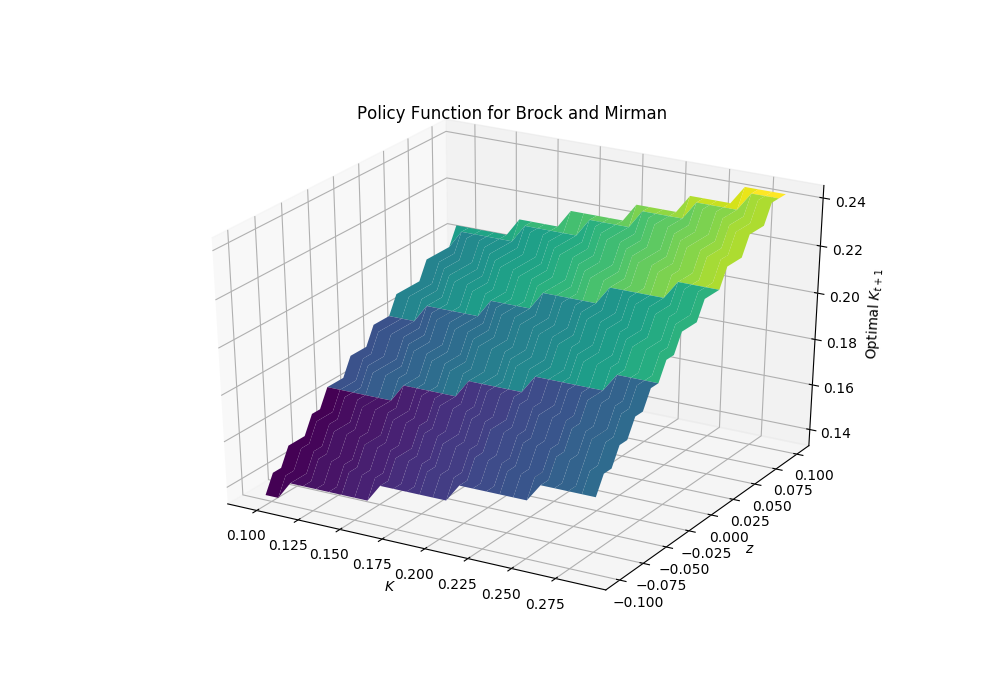
\includegraphics[width=\textwidth]{Brock_and_Merman_policy.png}
	\end{figure}

	% %9
	% \begin{Exercise} \label{DSGE_HW_BM_Grid_Log}
	% 	Repeat the above exercise using $k \equiv \ln K$ in place of $K$ as the endogenous state variable.
	% \end{Exercise}

	% %10
	% \begin{Exercise} \label{DSGE_HW_Base_Grid_Log}
	% 	Repeat the exercise \ref{DSGE_HW_BM_Grid} for the baseline tax model in section \ref{DSGE_SS_Base} using the same parameter values as in Exercise \ref{DSGE_HW_CES}.
	% \end{Exercise}

	% %11
	% \begin{Exercise} \label{Linear_HW_Base_Sims}
	% 	For the same model as above, generate 10,000 artificial time series for an economy where each time series is 250 periods long.  Start each simulation off with a starting value for $k$ equal to the steady state value, and a value of $z=0$.

	% 	Use $\sigma_z^2 = .0004$.

	% 	For each simulation save the time-series for GDP, consumption, investment, and the labor input.  When all 10,000 simulations have finished generate a graph for each of these time-series showing the average value over the simulations for each period, and also showing the five and ninety-five percent confidence bands for each series each period.
	% \end{Exercise}

	% % 12
	% \begin{Exercise} \label{Linear_HW_Base_Moments}
	% 	For the same model as above, calculate: the mean, volatility (standard deviation), coefficient of variation (mean divided by standard deviation), relative volatility (standard deviation divided bu the standard deviation of output), persistence (autocorrelation), and cyclicality (correlation with output); for each series over each simulation and report the average values and standard errors for these moments over the 10,000 simulations.
	% \end{Exercise}

	% % 13
	% \begin{Exercise} \label{Linear_HW_Base_IRFs}
	% 	For the same model as above, generate impulse response functions for: GDP, consumption, investment and total labor input; with lags from zero to forty periods.
	% \end{Exercise}


\section*{Linearization}\label{Linear_HW}

	\setcounter{Exercise}{0}
	% 1
	\begin{Exercise} \label{Linear_HW_BM_Coeffs}
		For the Brock and Mirman model in use Uhlig's notation to analytically find the values of the following matrices: $F, G, H, L, M$ \& $N$ as functions of the parameters.  Given these find the values of $P$ \& $Q$, also as functions of the parameters.  Imposing our calibrated parameter values, plot the three-dimensional surface plot for the policy function $K' = H(K,z)$.  Compare this with the closed form solution from the section \eqref{DSGE_BrockMirman} and the solution you found using the grid search method in exercise \ref{DSGE_HW_BM_Grid} frpom the DSGE chapter.
	\end{Exercise}

	Using section 1.4 and the fact that $\bar{K} = A^{\frac{1}{1-\alpha}} = (\alpha\beta)^{\frac{1}{1-\alpha}}$, we have that:

	\begin{align*}
		F &= \frac{\alpha\beta\bar{K}^{\alpha-1}}{\bar{K}^\alpha-\bar{K}} = 2.708 \\
		G &= -F(\alpha+\bar{K}^{\alpha-1}) = -8.843 \\
		H &= F(\alpha\bar{K}^{\alpha-1}) = 2.763 \\
		L &= -F\bar{K} = -0.522\\
		M &= F(\bar{K}^\alpha) = 1.522 \\
		N &= \rho - 0.95
	\end{align*}

	Now we can solve for $P$ and $Q$:
	\begin{align*}
		P &= \frac{-G \pm \sqrt{G^2-4FH}}{2F} = 0.35 \\
		Q &= -\frac{LN+M}{FN+FP+G} = 0.193
	\end{align*}

	Using the following linearized policy function $K_{t+1} = H(K_t,z_t) \bar{K}+P(K_t-\bar{K})+Qz_t$, we plot the three dimensional surface plot:

	\begin{figure}[H]
		\caption{Linearized Policy Function Given Current Capital Stock and Productivity Compared with Closed Form}
		\label{fig:brock_and_mirman}
		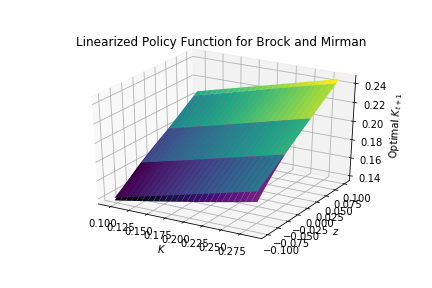
\includegraphics[width=0.8\textwidth]{Brock_and_Merman_linearized_policy.png}
	\end{figure}

	As seen, the linearized policy function intersects the real policy function (magma color scheme) at around the steady state ($K \approx 0.19, z = 0$) but deviates slightly at the non-linear parts.

	% 2
	\begin{Exercise} \label{Linear_HW_BM_Coeffs_Log}
		Repeat the above exercise using $k \equiv \ln K$ in place of $K$ as the endogenous state variable.
	\end{Exercise}

	We replace all values of $K$ in the Euler Equation with $e^k$. When taking the log-linearization of the new Euler Equation we get the following matrix values:
	\begin{align*}
		F&= -0.380254 \\
		G&= 0.468559 \\
		H&= -0.117414 \\
		L&= 2.569321 \\
		M&= -2.266718 \\
		N&=0.95 \\
		P&= 0.35 \\
		Q&= 6.756849
	\end{align*}

	% 3
	\begin{Exercise} \label{Linear_HW_Algebra}
		Do the necessary tedious matrix algebra necessary to transform equation \eqref{Linear_Approx3LogLin} into \eqref{Linear_Trans2LogLin}.
	\end{Exercise}

	Using the fact that $E\{\varepsilon_t\}=0$, we substitute equations (6), $\tilde{Z_t}=N\tilde{Z}_{t-1}$, and (7), $\tilde{X_t} = P\tilde{X}_{t-1}+Q\tilde{Z_t}$, into equation (5):
	\begin{align*}
		0 &= E_t\{F\tilde{X}_{t+1}+G\tilde{X_t}+H\tilde{X}_{t-1}+L\tilde{Z}_{t+1}+M\tilde{Z_t}\} \\
		&= FP\tilde{X_t}+FQN\tilde{Z}_{t}+GP\tilde{X}_{t-1}+GQ\tilde{Z_t}+H\tilde{X}_{t-1}+LN\tilde{Z}_{t}+M\tilde{Z_t} \\
		&= FPP\tilde{X}_{t-1}+FPQ\tilde{Z_t}+FQN\tilde{Z}_{t}+GP\tilde{X}_{t-1}+GQ\tilde{Z_t}+H\tilde{X}_{t-1}+LN\tilde{Z}_{t}+M\tilde{Z_t}\\
		&= [(FP+G)P+H]\tilde{X}_{t-1}+[(FQ+L)N+(FP+G)Q+M]\tilde{Z_t}
	\end{align*}

	% 4
	\begin{Exercise} \label{Linear_HW_Base_Numer_SS}
		For the baseline tax model, find the steady state values of $k$, $c$, $r$, $w$, $\ell$, $T$, $y$ and $i$, numerically.  Assuming $u(c_t,\ell_t) = \frac{c^{1-\gamma}_t -1}{1-\gamma}+ a \frac{(1-\ell_t)^{1-\xi}-1}{1-\xi}$ and $F(K_t,L_t,z_t) = K^{\alpha}_t (L_te^{z_t})^{1-\alpha} $.  Use the following parameter values: $\gamma = 2.5$, $\xi = 1.5$,  $\beta = .98$, $\alpha = .40$, $a=.5$, $\delta = .10$, $\bar z = 0$, $\rho_z=.9$ and $\tau = .05$.
	\end{Exercise}

	Note that in the steady state, $\bar{z} = 0$. Therefore, there is no uncertainty and the steady states when solved numerically are (this is the same as the DSGE exercise):
	\begin{align*}
		k&=4.225, \quad \ell= 0.580, \quad r= 0.121, \quad w=1.328, \quad c=0.861, \quad T=0.043, \quad y=1.283, \quad i=0.423
	\end{align*}

	% 5
	\begin{Exercise} \label{Linear_HW_Base_Numer_Deriv}
		For the same model as above, find $\frac{\partial y}{\partial x}$ for $y\in\{\bar k, \bar c, \bar r, \bar w, \bar \ell, \bar T, \bar y, \bar i\}$ and $x\in\{\delta, \tau, \bar z, \alpha, \gamma, \xi, \beta, a \}$ using numerical techniques.
	\end{Exercise}

	Using a first order central difference to estimate the derivatives, we have the following derivative matrix in the jupyter notebook output (refer to problem 5).

	% 6
	\begin{Exercise} \label{Linear_HW_Base_Coeffs}
		For the same model as above, let $X_t = \{k_{t-1}, \ell_t\}$.  Find the values of $F$, $G$, $H$, $L$, $M$, $N$, $P$ and $Q$.
	\end{Exercise}

	In order to coincide with the problem, we will use  $X_t = \{k_t,\ell_{t-1}\}$. In which case, the Uhlig's matrices are (for the log-linearized problem):
	\[
		F =
		\begin{bmatrix}
			-17.857 & 3.155\\
			0 & 0
		\end{bmatrix}
	\]

	\[
		G =
		\begin{bmatrix}
			36.196 & -3.254\\
			-22.527 & 8.638
		\end{bmatrix}
	\]

	\[
		H =
		\begin{bmatrix}
			-18.24 & 0 \\
			22.277 & 0
		\end{bmatrix}
	\]

	\[
		L =
		\begin{bmatrix}
			3.155 \\
			0
		\end{bmatrix}
	\]

	\[
		M =
		\begin{bmatrix}
			-3.254 \\
			3.004
		\end{bmatrix}
	\]

	\[
		P =
		\begin{bmatrix}
			0.915 & 0 \\
			-0.192 & 0
		\end{bmatrix}
	\]

	\[
		Q =
		\begin{bmatrix}
			0.129\\
			-0.011
		\end{bmatrix}
	\]

	% 7
	\begin{Exercise} \label{Linear_HW_Base_Sims}
		For the same model as above, generate 10,000 artificial time series for an economy where each time series is 250 periods long.  Start each simulation off with a starting value for $k$ equal to the steady state value, and a value of $z=0$.

		Use $\sigma_z^2 = .0004$.

		For each simulation save the time-series for GDP, consumption, investment, and the labor input.  When all 10,000 simulations have finished generate a graph for each of these time-series showing the average value over the simulations for each period, and also showing the five and ninety-five percent confidence bands for each series each period.
	\end{Exercise}

	\begin{figure}[H]
		\caption{GDP after 10,000 Simulations}
		\label{fig:GDP_10000}
		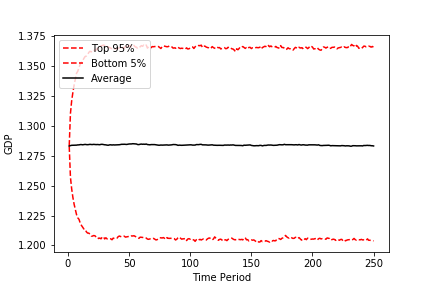
\includegraphics[width=0.7\textwidth]{GDP.png}
	\end{figure}

	\begin{figure}[H]
		\caption{Consumption after 10,000 Simulations}
		\label{fig:consumption_10000}
		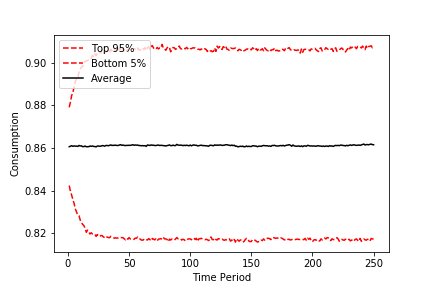
\includegraphics[width=0.7\textwidth]{consumption.png}
	\end{figure}

	\begin{figure}[H]
		\caption{Investment after 10,000 Simulations}
		\label{fig:investment_10000}
		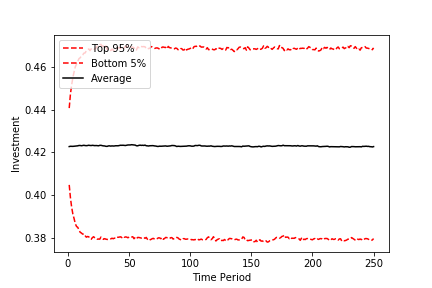
\includegraphics[width=0.7\textwidth]{investment.png}
	\end{figure}

	\begin{figure}[H]
		\caption{Labor after 10,000 Simulations}
		\label{fig:labor_10000}
		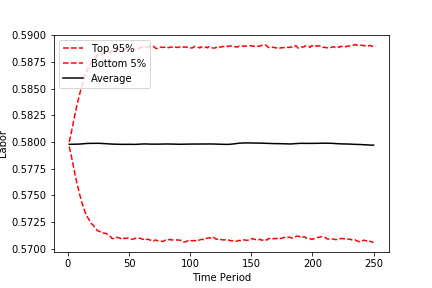
\includegraphics[width=0.7\textwidth]{labor.png}
	\end{figure}

	% 8
	\begin{Exercise} \label{Linear_HW_Base_Moments}
		For the same model as above, calculate: the mean, volatility (standard deviation), coefficient of variation (mean divided by standard deviation), relative volatility (standard deviation divided by the standard deviation of output), persistence (autocorrelation), and cyclicality (correlation with output); for each series over each simulation and report the average values and standard errors for these moments over the 10,000 simulations.
	\end{Exercise}

	Please refer to the juputer notebook for the result with all the moments.

	% 9
	\begin{Exercise} \label{Linear_HW_Base_IRFs}
		For the same model as above, generate impulse response functions for: GDP, consumption, investment and total labor input; with lags from zero to forty periods.
	\end{Exercise}

	\begin{figure}[H]
		\caption{Impulse Response of GDP}
		\label{fig:GDP_impulse}
		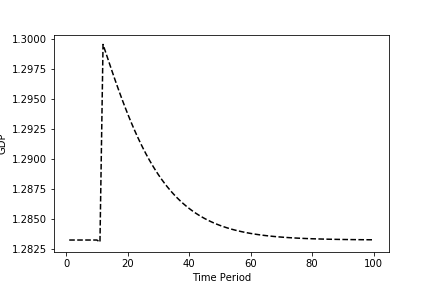
\includegraphics[width=0.7\textwidth]{GDPimpulse.png}
	\end{figure}

	\begin{figure}[H]
		\caption{Impulse Response of Consumption}
		\label{fig:consumption_impulse}
		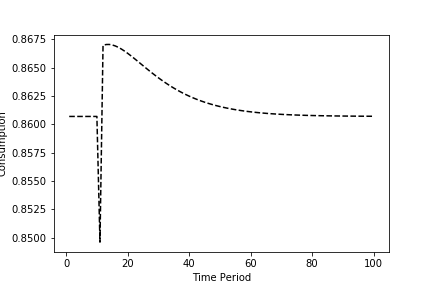
\includegraphics[width=0.7\textwidth]{Consumptionimpulse.png}
	\end{figure}

	\begin{figure}[H]
		\caption{Impulse Response of Investment}
		\label{fig:investment_impulse}
		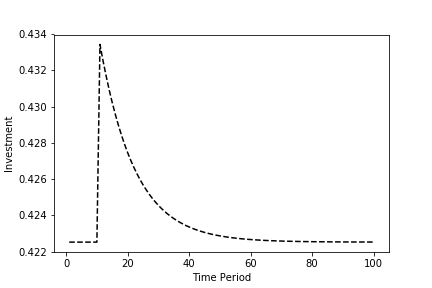
\includegraphics[width=0.7\textwidth]{Investmentimpulse.png}
	\end{figure}

	\begin{figure}[H]
		\caption{Impulse Response of Labor}
		\label{fig:labor_impulse}
		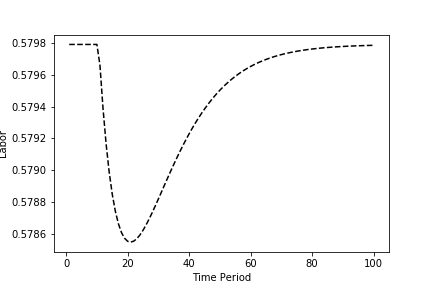
\includegraphics[width=0.7\textwidth]{Laborimpulse.png}
	\end{figure}

	% 10
	\begin{Exercise} \label{Linear_HW_OLG}
		Recall the TPI exercises from the OLG chapter.  Use the linear approximation methods from section \ref{Linear_LogLinApprox} to solve for the non-steady state equilibrium transition path of the economy from $(k_{2,1},k_{3,1})=(0.8\bar{k}_2,1.1\bar{k}_3)$ to the steady-state $(\bar{k}_2,\bar{k}_3)$. Use the same value for $T$ as you used when you solved the problem using time path iteration (TPI).  Plot the time paths for $k_2$, $k_3$ and $K$.  Compare the resulting time paths for the two methods.  Comment on the tradeoff between accuracy and compute time based upon this comparison.
	\end{Exercise}

	\begin{figure}[H]
		\caption{Transition Path for K2}
		\label{fig:k2_tpi}
		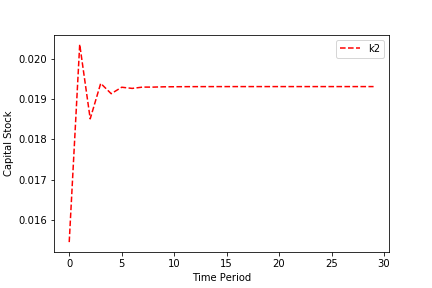
\includegraphics[width=0.7\textwidth]{k2TPI.png}
	\end{figure}

	\begin{figure}[H]
		\caption{Transition Path for K3}
		\label{fig:k3_tpi}
		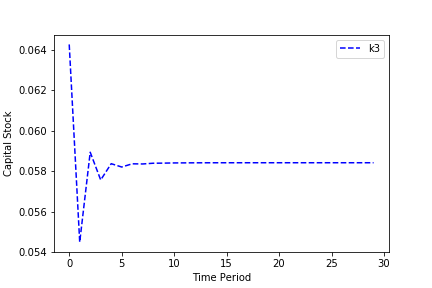
\includegraphics[width=0.7\textwidth]{k3TPI.png}
	\end{figure}

	\begin{figure}[H]
		\caption{Transition Path for K (Capital Stock)}
		\label{fig:K_tpi}
		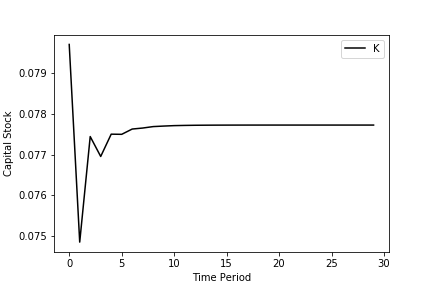
\includegraphics[width=0.7\textwidth]{KTPI.png}
	\end{figure}

	The graph for capital stock is very similar to the time path iteration result for capital, thus the linear approximation seems to be a good one. In this case, since the compute time is faster and more straight forward, it is a good tradeoff between accuracy and compute time.

	% 11
	\begin{Exercise} \label{Linear_HW_OLG_Stoch}
		Repeat the exercise above only this time assume there is a stochastic shock to the model, so that $A$ is replaced by $e^{z_t}$ with $z_t = \rho_z z_{t-1} + \epsilon_t;\,\epsilon_t \sim \text{i.i.d} (0,\sigma_z^2)$.  Let $\sigma_z=.02$ and $\rho_z=.9^{20}$.  As with exercise 9 above, run 10,000 simulations and report the average and confidence bands for GDP, total consumption and investment.
	\end{Exercise}

	\begin{figure}[H]
		\caption{GDP for OLG after 10,000 Simulations}
		\label{fig:GDP_OLG}
		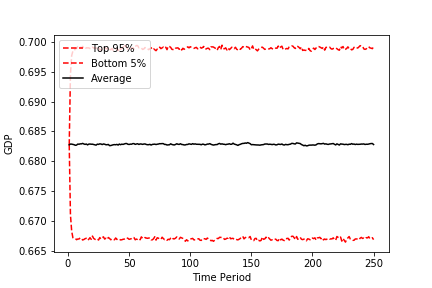
\includegraphics[width=0.7\textwidth]{GDP_OLG.png}
	\end{figure}

	\begin{figure}[H]
		\caption{Consumption for OLG after 10,000 Simulations}
		\label{fig:Consumption_OLG}
		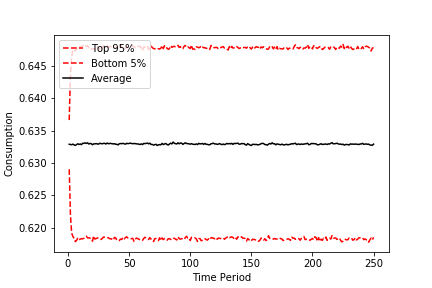
\includegraphics[width=0.7\textwidth]{Consumption_OLG.png}
	\end{figure}

	\begin{figure}[H]
		\caption{Investment for OLG after 10,000 Simulations}
		\label{fig:Investment_OLG}
		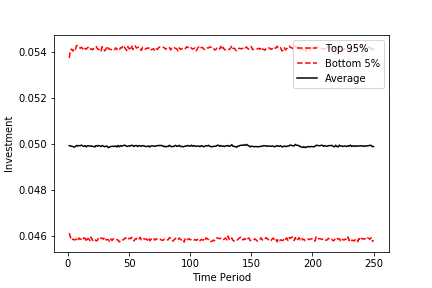
\includegraphics[width=0.7\textwidth]{Investment_OLG.png}
	\end{figure}

\section*{Perturbation}\label{Perturb_HW}
\setcounter{Exercise}{0}
	% 1
	\begin{Exercise} \label{Perturb_HW_Cubic}
		Following the example in equations \eqref{Perturb_Fxu2derv} and \eqref{Perturb_quad}, find the formula for the cubic term, $x_{uuu}(u_0)$, as a function of the derivatives of the $F$ function and the lower-order derrivatives of the $x$ function, i.e. $x(u_0)$, $x_u(u_0)$ and $x_{uu}(u_0)$.
	\end{Exercise}

	% 2
	\begin{Exercise} \label{Perturb_HW02_GEApprox}
		Consider the following static general equlibrim model.  Firms have a demand for labor curve given by $n^d = \left[\frac{(1-\alpha)z}{w}\right]^{\tfrac{1}{\alpha}} k$, where $z$ is the level of technology, $w$ is the wage rate, $k$ is a fixed capital stock, and $\alpha$ is a capital share parameter from a Cobb-Douglas production function.  Given this, the profits earned by the firm are $\pi = zk^\alpha (n^d)^{1-\alpha} - w n^d$.  The supply of labor by households is $n^s = h - \frac{b}{w(1+b)}(wh+\pi-t)$, where $h$ is the time endowment of the household, is $t$ is a lump-sum tax, and $b$ is a weight in utility on leisure versus consumption of goods.  Assuming a unit measure of both households and firms, use the following parameter values $\alpha = .33$, $k=5$, $z=1$, $b=2$, $t=.1$ and $h=24$.

		Find the market-clearing wage rate using {\tt fsolve}.  Find a first-order approxmation for wage as a function of $k$.  Approximate about $k=5$.

		Find a second-order approximation also about $k=5$.

		Set up a grid on the space between $k=1$ and $k=15$. Use {\tt fsolve} to find the equilibrium value of the wage at each point on the grid.

		Plot the grid solution, the linear and quadratic approximations on the same graph.

		Repeat the above exercise when the approximation point is $k=10$.
	\end{Exercise}

	% 3
	\begin{Exercise} \label{Perturb_HW_Bivar_Grid}
		For the function $F(y,x) =(x^{.35} + .9x - y)^{-2.5} - .95(y^{.35} + .9y )^{-2.5} = 0$, simplify and then use perturbation methods to find the cubic approximation of $y=G(x)$ about the point $x_0=100$.  In this case, $y_0=G(x_0)=10.5156$.

		Write out the functional form of this polynomial with numbers for coefficients.

		Set up a grid on the space between $x=99$ and $x=101$. Use {\tt fsolve} to find the equilibrium value of $y$ at each point on the grid.

		Plot the difference between the linear, quadratic and cubic approximations and the grid solution on the same graph over the range $x\in(99,101)$.
	\end{Exercise}

	% 4
	\begin{Exercise} \label{Perturb_HW_BM_NoStoch}
		For the \citet{BrockMirman1972} model in section \ref{Perturb_DGE} with the default parameter values find the scalar values of $H_X$ and $H_{XX}$.  Use analytical derivatives.

		Plot the the linear and quadratic approximations to policy function $K' = H(K)$.  Compare this with the closed form solution from the notes.
	\end{Exercise}

	% 5
	\begin{Exercise} \label{Perturb_HW_BM}
		For the \citet{BrockMirman1972} model with the default parameter values find the scalar values of $H_X$, $H_Z$, $H_{XX}$, $H_{XZ}$, $H_{ZZ}$ and $H_{vv}$.  Use numerical derivatives.

		Plot the three-dimensional surface plot for the policy function $K' = H(K,z)$.  Compare this with the closed form solution from the notes and the two approximations from the DSGE chapter Exercise 8 and the Linearization chapter Exercise 1.
	\end{Exercise}

	% 6
	% \begin{Exercise} \label{Perturb_HW_BAse}
	% 	Repeat Exercise \ref{Perturb_HW_BM} above using the baseline model from section 6 in the linearization chapter.  Generate figures similar to those you generated in the Linearization chapter in Exercise 7.  Compare this plot with the one from that exercise.
	% \end{Exercise}


\section*{Filtering}\label{Filter_HW}
\setcounter{Exercise}{0}
    % 1
    \begin{Exercise} \label{Filter_HW_CoVar_Proof}
        Prove that the spectral density of $X+Y$ is given by:
        $$S_X(\omega) + S_Y(\omega) + 2 Re(S_{XY}(\omega))$$
    \end{Exercise}

    % 2
    \begin{Exercise} \label{Filter_HW_HP_Proofs}
        Recall the minimization function for an HP filter is
        \begin{equation}\label{Filter_HW_HP_Proofs_eq01}
        \min_{g_t} \{ \sum_{t=1}^T (y_t - g_t)^2  +\lambda\sum_{t=2}^T[(g_{t+1}-g_{t}) - (g_{t}-g_{t-1})]^2\}
        \end{equation}

        Prove that as $\lambda \rightarrow \infty$, the filtered series $g_t$ is linear ($g_t = g_0 + \beta t$ for some $\beta$)

        Let $0 <\lambda < \infty$. What are the first order conditions for \ref{Filter_HW_HP_Proofs_eq01} for $t = 1, 2$ and the general case $k$?
    \end{Exercise}

    % 3
    \begin{Exercise} \label{Filter_HW_Periodograms}
        Find and plot the (non-smoothed) spectral density estimates for the following quarterly US time series: GDP, consumption, investment, and CPI.
    \end{Exercise}

    % 4
    \begin{Exercise} \label{Filter_HW_Periodograms_Filtered}
        Use the HP filter to filter the time series from Exercise \ref{Filter_HW_Periodograms} taking $\lambda = 1600$. Find and plot the spectral density estimates for both the trend and cyclical parts of the filtered time series.
    \end{Exercise}

    % 5
    \begin{Exercise} \label{Filter_HW_Moments_HP}
        Using the data from Exercise \ref{Filter_HW_Periodograms}, filter each series using the HP filter with values of $\lambda=\{100,400,1600,6400,25600\}$.  For each series and each value of $\lambda$,
        calculate the mean, standard deviation, autocorrelation, and correlation with GDP.  Report these values an comment on the results.  Plot the time-series for output along with the 5 smoothed series.
    \end{Exercise}

    % 6
    \begin{Exercise} \label{Filter_HW_Moments}
        Replicate Table \ref{Stylized_USData_Tab} using data collected from the sites mentioned in Section \ref{Sec_FindData}.  Use quarterly data going back as far as 1947, if possible.  Do this for each of the following filters:
        \begin{itemize}
          \setlength\itemsep{0em}
          \item A linear trend filter
          \item the first difference ($y_t - y_{t-1}$) filter
          \item HP($\lambda=1600$)
          \item BP(6,32,$K=8$)
        \end{itemize}
    \end{Exercise}

\end{spacing}

\newpage

\bibliography{BootCampText}

\end{document}
